%%
%% Vehicular Communications submission
%% Converted from MDPI Remote Sensing submission
%% Journal: Vehicular Communications (Elsevier)
%%
\documentclass[preprint,12pt]{elsarticle}

%% Packages
\usepackage{amssymb}
\usepackage{amsmath}
\usepackage{graphicx}
\usepackage{algorithm}
\usepackage{algpseudocode}
\usepackage{booktabs}
\usepackage{multirow}
\usepackage{array}
\usepackage{tabularx}
\usepackage{microtype}
\setlength{\emergencystretch}{2em}

%% Configure algorithm environment
\floatname{algorithm}{Algorithm}

%% Breakable arrow for tables
\newcommand{\arw}{$\rightarrow$\allowbreak\hspace{0pt}}

%% Journal name
\journal{Vehicular Communications}

\begin{document}

\begin{frontmatter}

%% Title
\title{Risk-Aware Predictive Vertical Handover for UAV Communications in Heterogeneous Wireless Networks}

%% Authors with affiliations
\author[jnu]{Hanming Sun}
\ead{202210043@jnxy.edu.cn}

\author[cdut]{Tong Liu\corref{cor1}}
\ead{liutong1982@cdut.edu.cn}

\author[cdut]{Wen Su}
\ead{suwen@stu.cdut.edu.cn}

\author[cdut]{Jie Lin}
\ead{linjie07@cdut.edu.cn}

\author[cdut]{Junsong Luo}
\ead{luojuns@cdut.edu.cn}

\author[jniit]{Yu Tian}
\ead{ytian@jniit.com.cn}

\author[jniit]{Wenshu Sun}
\ead{wssun@jniit.com.cn}

\author[cdut]{Bin Duo}
\ead{duobin@cdut.edu.cn}

%% Corresponding author
\cortext[cor1]{Corresponding author}

%% Affiliations
\affiliation[jnu]{organization={School of Mechanical and Electrical Engineering, Jining University},
            city={Jining City},
            postcode={273155},
            state={Shandong Province},
            country={China}}

\affiliation[cdut]{organization={School of Computer and Network Security, Chengdu University of Technology},
            city={Chengdu},
            postcode={610059},
            country={China}}

\affiliation[jniit]{organization={Jining Institute of Industrial Technology},
            city={Jining},
            postcode={272000},
            country={China}}

%% Abstract (approx 200 words, self-contained)
\begin{abstract}
Unmanned aerial vehicles must select among heterogeneous access networks while maintaining time-sensitive telemetry and image delivery. This study develops a task-conditioned predictive vertical-handover framework combining stacked LSTM forecasting, learned attention-based attribute weights, TOPSIS ranking, and persistent handover confirmation. A risk-aware extension adapts the score margin and penalizes uncertain candidates using residual variability. A three-stage mission comprises departure through a 5G NR region, slow imaging near a Wi-Fi station, and LTE-supported return. The simulator uses actual NR, LTE and Wi-Fi protocol stacks, a shared upstream payload process, packet-level deadlines and explicit application-layer service migration. An independent service-model optimizer evaluates unrestricted network sequences and switching costs. Three development missions support two service-reference transitions, providing a controlled setting for paired packet-level evaluation and prediction ablations.
\end{abstract}

%% Keywords
\begin{keyword}
UAV communications \sep heterogeneous wireless networks \sep vertical handover decision \sep network selection \sep LSTM \sep attention mechanism
\end{keyword}

\end{frontmatter}
\normalsize

\section{Introduction}\label{sec:intro}

Unmanned aerial vehicles (UAVs) are increasingly deployed in heterogeneous wireless network environments, where multiple radio access technologies—including fifth-generation (5G), Long-Term Evolution (LTE), and Wi-Fi—coexist with overlapping coverage areas. UAV mobility introduces unique vertical handover (VHO) challenges that differ fundamentally from ground-based scenarios: rapid altitude changes, high-speed boundary crossings, and three-dimensional trajectory variations create dynamic channel conditions that demand intelligent network selection strategies. The core technical challenge lies in managing seamless connectivity across coverage boundaries while maintaining quality of service for real-time aerial data transmission \cite{ref1,ref2,ref3}. This study addresses the network selection decision problem: determining when to initiate a handover and which target network to select, based on predicted channel conditions and dynamic attribute weighting. Existing VHO methods mainly employ multiple attribute decision making (MADM) \cite{ref7}, including the technique for order preference by similarity to the ideal solution (TOPSIS) \cite{ref8,ref9,ref10}, VIsekriterijumska Optimizacija I Kompromisno Resenje (VIKOR) \cite{ref11}, and the Grey relational analysis (GRA), complex proportional assessment (COPRAS), stable preference ordering toward ideal solution (SPOTIS), and simple additive weighting (SAW) methods \cite{ref12}. Beyond deterministic MADM frameworks, fuzzy-logic-based approaches such as Fuzzy-VHO apply fuzzy inference to handle uncertain channel measurements and handover decisions \cite{ref4}. More recently, deep reinforcement learning (DRL) methods have been explored to learn adaptive handover policies from experience \cite{ref16,ref17,ref18}. Despite their different formulations, these approaches have common limitations. MADM and fuzzy methods typically use fixed weights—often derived from entropy weighting or the analytic hierarchy process \cite{ref12,ref13,ref14,ref15}—limiting adaptation to varying flight phases and channel conditions, and rely on current network indicators without predicting future states, potentially delaying handovers until link failure when a UAV approaches coverage limits \cite{ref16,ref17}. DRL-based methods remain limited by black-box decision-making and unstable training, which undermine interpretability and reliability in safety-critical aerial missions.

LSTM networks alleviate vanishing gradients through gated structures \cite{ref19} and capture long-range temporal dependencies; they have accordingly been used to forecast handover-related network states in 5G heterogeneous networks \cite{ref20,ref21,ref22}. Because such forecasting is trained by supervised regression against measured next-period states, it can be inserted into a multi-attribute decision framework as an explicit prediction stage, without replacing the decision rule by a learned policy. In existing schemes, however, the forecast serves mainly to refresh the indicator values that enter the decision layer, whereas the weights and thresholds of that layer are still specified offline; the benefit is therefore confined to smoother inputs rather than adaptive decision logic.

VHO in UAV heterogeneous wireless networks involves two challenges. The first is informational. Conventional MADM ranks candidates on instantaneous indicators and therefore cannot anticipate a link that is about to fail, and although a single LSTM can forecast the next-period state, existing designs use that forecast only to refresh the indicators while leaving the decision rule untouched: the forecast changes what is known, not how the decision is made. The second is parametric. Attribute weights are fixed using entropy weighting or the analytic hierarchy process \cite{ref12,ref13,ref14,ref15}, and the score margin and confirmation window are held constant, yet the relative importance of SINR, delay, throughput, and packet loss differs between cruise and imaging phases, and the channel is quiescent in steady flight but fluctuates sharply near coverage boundaries and obstacles. A margin lax enough to avoid chattering in steady flight responds to boundary noise, while one strict enough to suppress that noise delays necessary handovers, and the same tension governs the length of the confirmation window. Handover instability therefore stems less from limited sensing than from decision logic whose parameters cannot follow the flight state. Addressing these challenges requires a framework that integrates temporal prediction with adaptive decision parameters.

To address these challenges, LAAVHA combines multihorizon LSTM forecasting, task-conditioned attention weights, fused-state TOPSIS and persistent handover confirmation. The prediction stage anticipates changes in candidate service; learned weights respond to network state, speed, altitude and current application demand. A causal forecast-error check reduces reliance on uncertain predictions. A separate recovery path responds to serving-link failure. ALERA extends the score rule with a residual-variability penalty and a margin adapted to detrended SINR increments. The evaluation measures whether these mechanisms preserve timely telemetry and image delivery while avoiding transient intermediate migrations.

The evaluation connects predictive selection to task-level service outcomes. An independent service-reference optimizer compares unrestricted network sequences and explicit migration costs, while paired physical integration missions measure telemetry deadline delivery, image goodput and interruption. This evaluation distinguishes timely, useful migration from a low switch count obtained by retaining an unsuitable link.


\section{Mission Scenario and Measurement Model}\label{sec:scenario}
The mission occupies a $2000\times2000$ m region. The NR gNB, LTE eNB and Wi-Fi access point are located at $(1500,1000,30)$, $(700,1000,30)$ and $(1000,1000,10)$ m, respectively. The UAV starts near $(1600,1000,100)$ m and flies west. Its nominal horizontal speed is 30 m/s during departure, 5 m/s near the imaging station, and 25 m/s during return, with one-second continuous transitions. Position and altitude perturbations are sampled once per mission. Figure~\ref{fig:network_coverage} is generated from the executable mission configuration.
\begin{figure}[ht]\centering
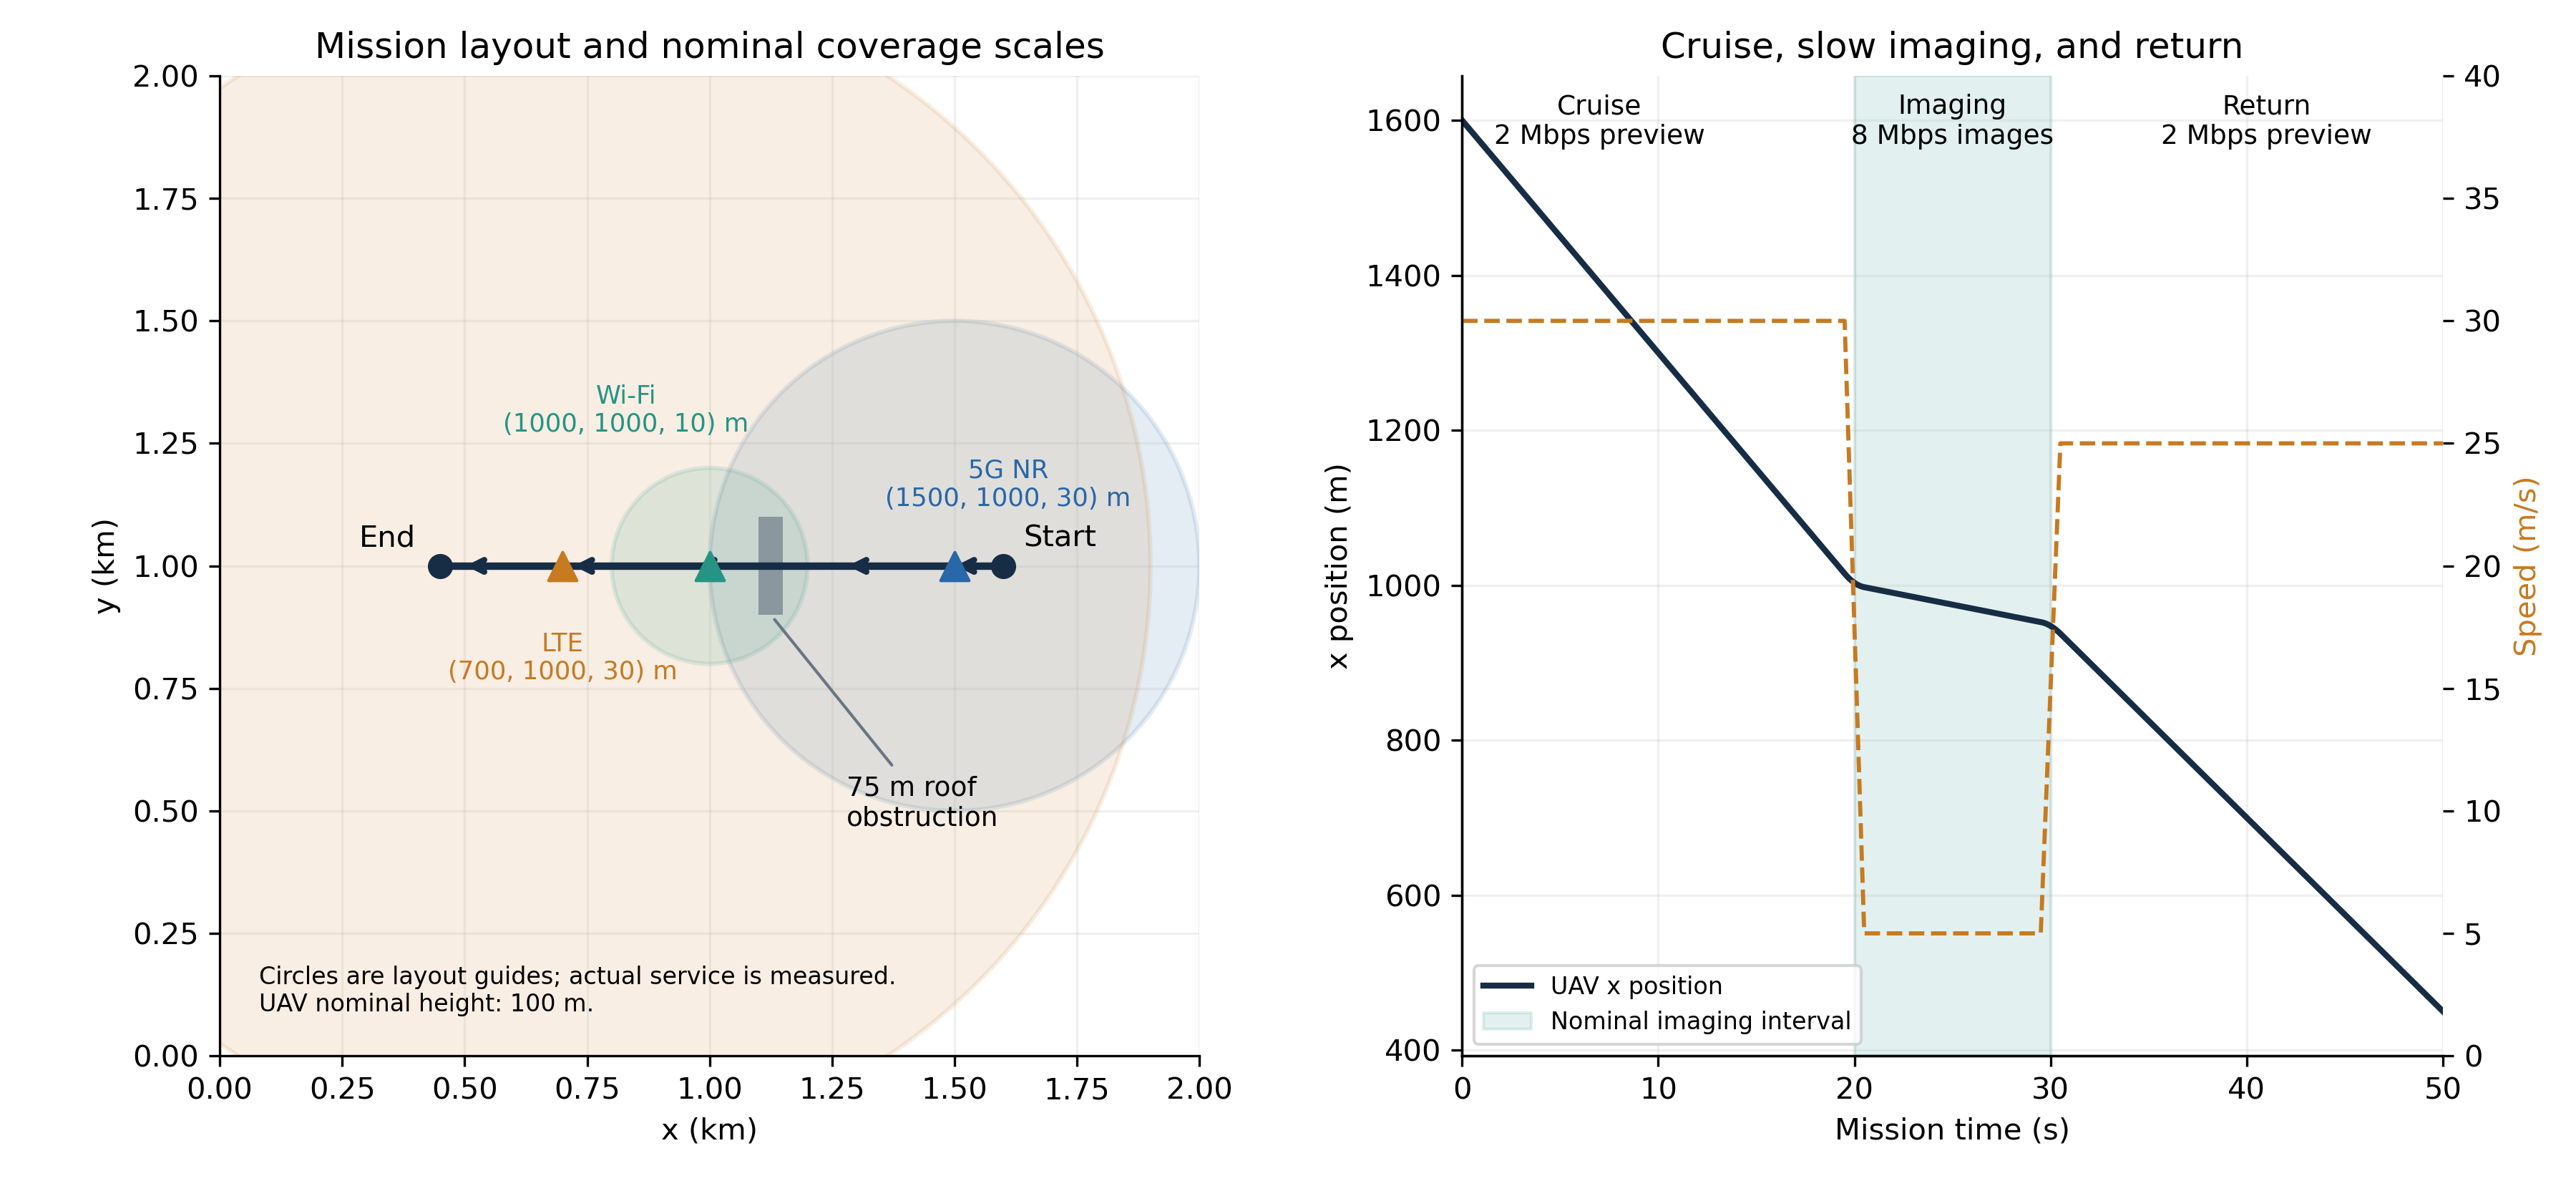
\includegraphics[width=\textwidth]{Figures/fig1_mission_v2.png}
\caption{Three-stage mission, geometric obstruction and nominal coverage scales. Coverage circles guide layout and do not impose receiver availability or switching times.}
\label{fig:network_coverage}\end{figure}
The application generates 64 kbps telemetry throughout the mission, with a 50 ms deadline. Preview traffic is 2 Mbps; within the geographic imaging interval $950\leq x\leq1000$ m, image traffic is 8 Mbps. Video/image packets have a 200 ms deadline. Every policy receives the same current task requirement. All traffic is upstream to a common server, and payload generation is independent of the selected network.

The physical platform comprises ns-3.45, 5G-LENA v4.1, LTE/EPC and 802.11n Wi-Fi. The engineering propagation model uses log-distance exponents 2.8, 3.1 and 3.0 for NR, LTE and Wi-Fi, with respective 1 m reference losses of 43.3, 38 and 40 dB. This is a declared engineering air-link model rather than a validated TR38.901 UAV channel. A building spanning $x=1100$--1150 m, $y=900$--1100 m and $z=0$--75 m introduces an 18 dB loss when a propagation ray intersects it. This loss acts on actual radio power. Its value is subject to sensitivity evaluation. LTE has a declared 6 Mbps backhaul allocation. The same physical assumptions apply to every policy.

Three co-moving radio-endpoint nodes represent one logical UAV. The application coordinator sends each payload packet through one endpoint only. A service migration changes that endpoint and introduces a modeled 100 ms application interruption; packets generated during that interval are counted as interruption losses. The implementation does not execute a cross-RAT attach procedure and does not interpret the interruption parameter as measured protocol latency. Interfaces are connected and probed during a two-second warmup; the 50 s mission begins with verified NR service.

Candidate observations comprise receiver SINR, received reference power/RSSI, probe delay, a PHY-based available-capacity estimate, and probe deadline loss. These estimates are distinct from payload goodput. Probes use shared generation intervals and their own packet cohorts. A cohort is evaluated only after its deadline; in-flight packets are not counted as lost. A missing delay is explicitly flagged and mapped to a conservative representation. Actual telemetry and image outcomes are computed from unique payload identifiers and application generation/receive timestamps, followed by a one-second drain interval.

\section{Task-Conditioned LAAVHA and ALERA}\label{sec:laavha}
Each candidate contributes ten historical states separated by 0.1 s. Two LSTM layers, with 128 and 64 hidden units, forecast the five indicators at horizons 0.1, 0.3 and 0.5 s. The same physical clipping applies before training and inference: SINR is bounded to $[-50,80]$ dB, received power to $[-180,-10]$ dBm, delay to $[0,1000]$ ms, estimated capacity to $[0,200]$ Mbps and loss to $[0,1]$. Below-floor native reference-power values enter as the conservative lower bound. Training means and standard deviations are fitted on whole training missions and stored with the checkpoint. A causal forecast-error check guards inference. The score-fusion stage uses the 0.3 s prediction and falls back toward current measurements when recent forecast errors are large.

The weighting branch embeds current network states into 16-dimensional vectors, applies single-head self-attention, pools across candidates and concatenates normalized speed, altitude and current traffic demand. A trained projection produces five attribute weights:
\begin{equation}w_j=0.04+0.8\,\mathrm{softmax}(z)_j.\end{equation}
The floor prevents an attribute from being completely discarded. The training loss combines normalized multihorizon prediction MSE, candidate-ranking supervision from a fixed external service objective, and weight regularization. Both prediction and weighting branches receive gradients. Validation selects checkpoints using prediction and ranking loss; adjacent windows from one mission are never split across training and validation.
\begin{equation}
\mathcal L=\mathcal L_{\mathrm{pred}}-\frac1N\sum_{n,i}p_{ni}\log q_{ni}
+0.1\frac1{5N}\sum_{n,j}(w_{nj}-0.2)^2,
\end{equation}
where $p_{ni}$ is the softmax distribution of external service values at temperature 0.1 and $q_{ni}$ is the softmax distribution of weighted TOPSIS scores at the same temperature. Training uses complete missions 0--7; validation uses missions 100 and 101. Adam uses learning rate 0.001 and batch size 128 for 35 epochs, with validation checkpoint selection.
\begin{table}[ht]\centering\small
\caption{Prediction validation on two complete missions, seeds 100 and 101. MSE is normalized with training-mission attribute scales.}
\label{tab:prediction}
\begin{tabular}{rrrr}\hline
Horizon (s) & LSTM & Persistence & Linear trend \\ \hline
0.1 & 0.007952 & 0.007043 & 0.009672 \\
0.3 & 0.018065 & 0.025546 & 0.053357 \\
0.5 & 0.031674 & 0.046605 & 0.130642 \\
\hline\end{tabular}\end{table}


Fixed engineering transforms map the five indicators to benefit features. For current video demand $d$, the benefit features are
\begin{equation}
f(S,d)=\operatorname{clip}_{[0,1]}\left[
\frac{\mathrm{SINR}+10}{40},\frac{P+120}{70},
e^{-D/50},\min(C/d,1),1-L\right].
\end{equation}
Here $P$ is received reference power or RSSI in dBm, $D$ is probe delay in ms, $C$ is estimated capacity in Mbps, and $L$ is probe deadline loss. The nominal current-state coefficient is $\alpha=0.6$. If $e_t$ is the mean absolute feature error of the previous one-step forecast, confidence is $c_t=e^{-e_t/0.15}$ and the effective current-state coefficient is $a_t=1-(1-\alpha)c_t$. Thus low confidence shifts the fused features toward observations. Weighted TOPSIS computes candidate closeness from $a_t f(S_t,d_t)+(1-a_t)f(\hat S_{t+0.3},d_t)$. Normal migration requires a score advantage exceeding 0.03 for three consecutive decisions.

All compared policies share the same declared availability guard. A candidate must show recent service capacity of at least 0.1 Mbps, delay within 200 ms and loss below 0.5. Normal predictive migration additionally checks whether the 0.3 s and 0.5 s forecast rankings agree on a persistent destination. Such a destination must already be usable and better than the serving network; otherwise the policy defers a potentially short-lived intermediate migration. The same check is applied to simple predictive controls. When the serving link fails and another is usable, a two-step recovery rule overrides normal score hysteresis and predictive deferral. When all candidates are unavailable the policy retains its current interface and records outage. No policy receives a desired network order, a route-specific switching time or a handover-count limit.

ALERA subtracts a risk term based on recent score increments and adjusts the margin using detrended SINR increments. This distinguishes stochastic variation from a monotonic degradation trend. The implementation retains separate no-prediction and no-attention variants. Strong controls include task-weighted TOPSIS with the same guards and hysteresis, five-sample moving-average and linear prediction controls, strongest-SINR selection, and adapted MADM alternatives. The task-aware control uses weights (0.10,0.05,0.25,0.30,0.30) for preview and (0.05,0.05,0.15,0.45,0.30) for imaging, in the declared attribute order. This provides a direct test of whether learned weights add value. The moving-average control retains the historical CLI identifier \texttt{ewma}; its averaging window has uniform weights.
\begin{align}
\widetilde C_i(t)&=C_i(t)-0.5\operatorname{std}\{\Delta C_i\},\\
\Delta_{\mathrm{ALERA}}(t)&=0.03+
\min\left(0.05,\,0.005\operatorname{std}\{\Delta\mathrm{SINR}_{\mathrm{serving}}\}\right).
\end{align}
Both standard deviations use increments within the five most recent samples; the score history stores values before risk correction. A linear decline therefore contributes little residual variability. ALERA retains three-step normal confirmation and the shared two-step failure recovery.

\begin{algorithm}[ht]
\caption{Causal mission-conditioned LAAVHA selection}
\begin{algorithmic}[1]
\Require Historical candidate observations, current task demand and mobility, serving interface, confirmation state
\State Clip observations and update the ten-sample history
\State Forecast 0.1/0.3/0.5 s states and generate trained task-conditioned weights
\State Estimate confidence using the preceding one-step forecast error
\State Fuse current and 0.3 s benefit features; compute weighted TOPSIS scores
\State Apply ALERA residual correction when that variant is enabled
\State Determine usable candidates from recent capacity, delay and loss
\If{no candidate is usable}
  \State Keep serving interface and record unavailable service
\ElsIf{serving interface is unusable}
  \State Confirm a usable alternative for two decisions, then migrate
\Else
  \State Check agreement of 0.3/0.5 s forecast destinations
  \State Confirm a persistent usable score advantage for three decisions
  \State Migrate when confirmation and interruption constraints permit
\EndIf
\end{algorithmic}
\end{algorithm}

\section{Independent Reference and Validation}\label{sec:sim}
The offline reference uses an external task objective rather than TOPSIS closeness or learned weights. In its declared fresh-cohort service model, telemetry consumes capacity first, remaining capacity serves video, and cohorts missing their deadline yield no service. Telemetry satisfaction has weight four and video satisfaction weight one; an explicit switch cost is subtracted. A dynamic program tracks the serving network, interruption state and optional switch-count budget. It optimizes arbitrary network orders and counts. It is checked against exhaustive enumeration on short sequences.

The external objective is
\begin{equation}
J=\sum_t \bigl(4s_{\mathrm{telemetry},t}+s_{\mathrm{video},t}\bigr)
(1-\ell_t/\Delta t)\Delta t-0.02H,
\end{equation}
where satisfaction values follow priority capacity allocation and the respective deadlines, $\ell_t$ is the service time lost to migration in the slot, $\Delta t=0.1$ s and $H$ is the raw switch count. The reference is exact for this fresh-cohort service model. Physical packet queues and policy-dependent observations are evaluated separately by ns-3 replay.
\begin{table}[ht]\centering\small
\caption{Independent fresh-cohort service reference on fixed-NR calibration observations. The objective includes modeled interruption and switching cost. Columns 0--2 impose at most that many switches; the unrestricted solution has no count limit.}
\label{tab:reference}
\begin{tabular}{rrrrrr}\hline
Seed & 0 & 1 & 2 & Unrestricted & Count \\ \hline
100 & 149.1549 & 247.6234 & 248.9600 & 248.9600 & 2 \\
108 & 169.4272 & 248.6509 & 248.9600 & 248.9600 & 2 \\
119 & 143.7300 & 248.3344 & 248.9600 & 248.9600 & 2 \\
\hline\end{tabular}\end{table}
The two-switch optimum exceeds every zero- or one-switch solution in these calibration missions. Allowing additional switches does not improve the objective. The selected sequence is NR--Wi-Fi--LTE. This result follows from the measured candidate service estimates and the declared objective.

\begin{table}[ht]\centering\small
\caption{Packet-level replay of schedules obtained from fixed-NR calibration, seed 100. Both schedules are offline references with access to future candidate estimates.}
\label{tab:packet_reference}
\setlength{\tabcolsep}{4pt}
\begin{tabular}{lrrrr}\hline
Schedule & Switches & Telemetry (\%) & Video (\%) & Goodput (Mbps) \\ \hline
One-switch reference & 1 & 86.30 & 70.72 & 2.124 \\
Two-switch reference & 2 & 99.20 & 99.01 & 2.973 \\
\hline\end{tabular}\end{table}
The two-switch reference supplies the imaging stage through Wi-Fi and preserves substantially more deadline-qualified service in this replay.

Sensitivity evaluates switch costs 0.005/0.02/0.05 and interruption durations 0/0.05/0.1/0.2 s. Stress missions allow different reference counts, including an archived 85 m roof configuration whose coverage gap requires an intermediate LTE migration.

Physical integration pilots cover 3 mission seeds. Table~\ref{tab:pilot} reports their descriptive means. These seeds were used during development; they provide no held-out generalization estimate. LAAVHA records raw switch counts of 2, 2, 2, with mean telemetry and video deadline delivery of 98.67\% and 99.01\%, respectively.

\begin{table}[ht]
\centering\small
\caption{Physical integration pilots. These missions are development evidence, not the held-out benchmark. Delivery denotes the fraction of generated payload packets received by their deadlines.}
\label{tab:pilot}
\begin{tabular}{lrrrr}\hline
Method & Missions & Switches & Telemetry (\%) & Video (\%) \\ \hline
alera & 3 & 2.00 & 98.67 & 99.01 \\
moving-average & 3 & 2.00 & 98.20 & 98.67 \\
laavha & 3 & 2.00 & 98.67 & 99.01 \\
no-attention & 3 & 2.00 & 98.53 & 98.90 \\
no-pred & 3 & 2.00 & 98.60 & 98.96 \\
strongest-SINR & 3 & 2.33 & 98.13 & 98.62 \\
topsis & 3 & 2.00 & 98.40 & 98.81 \\
trend & 3 & 2.00 & 98.53 & 98.90 \\
\hline\end{tabular}
\end{table}

\begin{figure}[ht]\centering
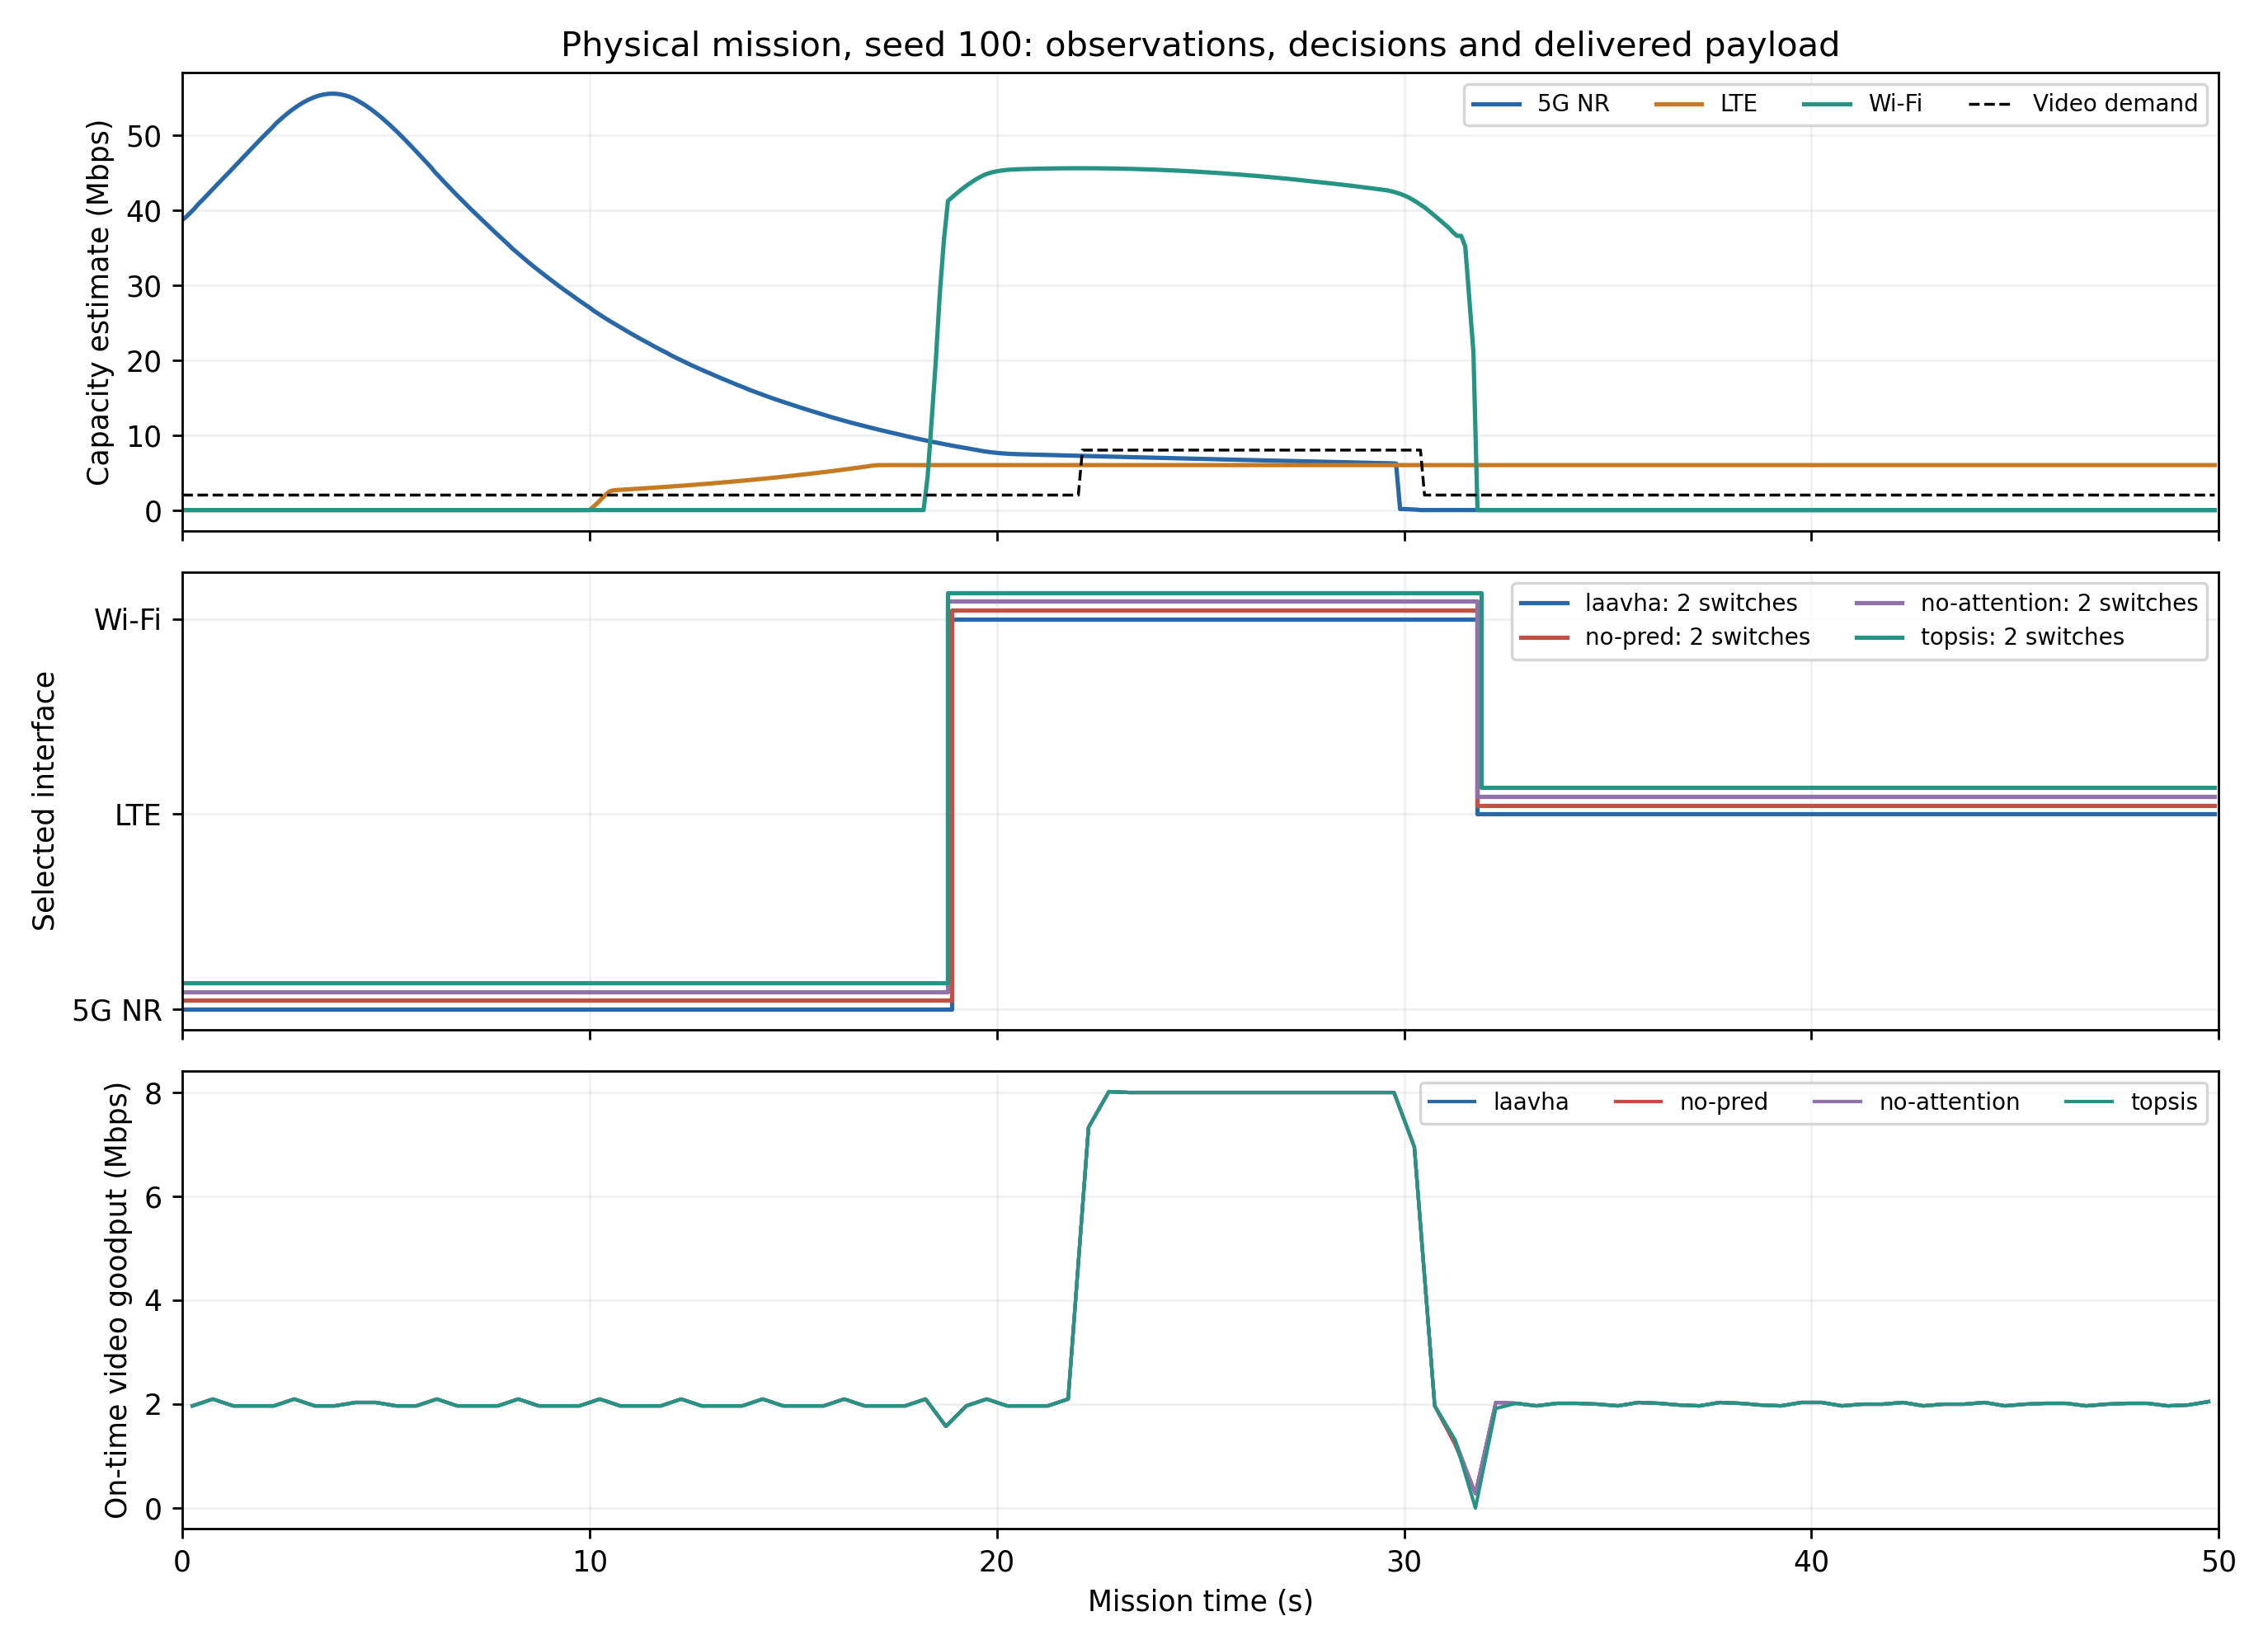
\includegraphics[width=\textwidth]{Figures/physical_timeline_seed100.png}
\caption{Physical pilot observations, selected interfaces and deadline-qualified video goodput for seed 100. Capacity estimates are used for decisions; the bottom panel is computed from received payload packets. Small vertical offsets distinguish coincident interface sequences.}
\label{fig:physical_timeline}\end{figure}
Primary measured outcomes are telemetry deadline delivery, image deadline goodput, payload delay percentiles, service-interruption losses and raw application migration count. An additional zero-delivery-cohort measure counts generation windows in which no payload packet subsequently arrives by its deadline. Repeated-seed summaries use missions as independent units. The integration comparison includes shared-guard task TOPSIS, simple prediction controls and component ablations.

\section{Conclusion}\label{sec:conclusion}
Task-conditioned LAAVHA connects predictive network selection to telemetry deadlines and image demand. The three-stage mission supports an independently evaluated two-transition service reference, while causal confidence checks, persistent destination selection and failure recovery govern online migration. Paired integration missions and component ablations expose the relationship between raw switching count and delivered payload. Further evaluation will quantify performance across held-out missions, background traffic and broader geometries.

\section*{CRediT authorship contribution statement}

\textbf{Hanming Sun}: Conceptualization, Methodology, Software, Validation, Formal analysis, Writing -- original draft.
\textbf{Tong Liu}: Conceptualization, Supervision, Writing -- review \& editing, Funding acquisition.
\textbf{Wen Su}: Software, Validation, Writing -- review \& editing.
\textbf{Jie Lin}: Formal analysis, Writing -- review \& editing.
\textbf{Junsong Luo}: Investigation, Writing -- review \& editing.
\textbf{Yu Tian}: Resources, Writing -- review \& editing.
\textbf{Wenshu Sun}: Data curation, Writing -- review \& editing.
\textbf{Bin Duo}: Supervision, Project administration, Funding acquisition.

\section*{Declaration of competing interest}

The authors declare that they have no known competing financial interests or personal relationships that could have appeared to influence the work reported in this paper.

\section*{Data availability}

The simulation code and trained model weights supporting the findings of this study are available from the corresponding author upon reasonable request. Raw simulation data cannot be publicly deposited due to the large file size of ns-3 trajectory outputs.

\section*{Acknowledgements}

The authors thank the anonymous reviewers for their constructive comments.

%=================================================================
%% References
\begin{thebibliography}{999}
\bibitem{ref1}
K. Yang, Y. Wang, X. Gao, et al., Communications in space--air--ground integrated networks: An overview, Space Sci. Technol. 5 (2025) 0199.

\bibitem{ref2}
G. Geraci, A. García-Rodríguez, M.M. Azari, et al., What will the future of UAV cellular communications be? A flight from 5G to 6G, IEEE Commun. Surv. Tutor. 24 (2022) 1304--1335. https://doi.org/10.1109/COMST.2022.3171135.

\bibitem{ref3}
L.M.B. Ribeiro, I. Müller, L.B. Becker, Communication interface manager for improving performance of heterogeneous UAV networks, Sensors 21 (2021) 4255.

\bibitem{ref4}
T. Ayass, T. Coqueiro, T. Carvalho, et al., Unmanned aerial vehicle with handover management fuzzy system for 5G networks: Challenges and perspectives, Intell. Robot. 2 (2022) 20--36.

\bibitem{ref5}
A.U. Rehman, M.B. Roslee, J.J. Tiang, A survey of handover management in mobile HetNets: Current challenges and future directions, Appl. Sci. 13 (2023) 3367.

\bibitem{ref6}
A. Haghrah, M.P. Abdollahi, H. Azarhava, et al., A survey on the handover management in 5G-NR cellular networks: Aspects, approaches and challenges, EURASIP J. Wirel. Commun. Netw. 2023 (2023) 52.

\bibitem{ref7}
Z. Wang, Z. Lv, X. Xu, et al., Vertical switching algorithm for unmanned aerial vehicle in power grid heterogeneous communication networks, Electronics 13 (2024) 2612.

\bibitem{ref8}
J. Zhong, L. Zhang, M. Alhabo, et al., A hybrid scheme using TOPSIS and Q-learning for handover decision making in UAV-assisted heterogeneous network, IEEE Access 12 (2024) 31422--31430. https://doi.org/10.1109/ACCESS.2024.3368916.

\bibitem{ref9}
M.I. Goh, A.I. Mbulwa, H.T. Yew, et al., Handover decision-making algorithm for 5G heterogeneous networks, Electronics 12 (2023) 2384.

\bibitem{ref10}
C.L. Hwang, K. Yoon, Multiple Attribute Decision Making: Methods and Applications. A State-of-the-Art Survey, Springer-Verlag, Berlin, Germany, 1981.

\bibitem{ref11}
S. Zolfani, M. Yazdani, D. Pamucar, et al., A VIKOR and TOPSIS focused reanalysis of the MADM methods based on logarithmic normalization, Facta Univ. Ser. Mech. Eng. 18 (2020) 341--355.

\bibitem{ref12}
F.S. Dantas Silva, M.P.S. Lima, D. Corujo, et al., A comprehensive step-wise survey of multiple attribute decision-making mobility approaches, IEEE Access 12 (2024) 108616--108656. https://doi.org/10.1109/ACCESS.2024.3436074.

\bibitem{ref13}
P. Satapathy, J. Mahapatro, An efficient multicriteria-based vertical handover decision-making algorithm for heterogeneous networks, Trans. Emerg. Telecommun. Technol. 33 (2022) e4409.

\bibitem{ref14}
Y. Zhong, H. Wang, H. Lv, et al., A vertical handover decision scheme using subjective-objective weighting and grey relational analysis in cognitive heterogeneous networks, Ad Hoc Netw. 134 (2022) 102924.

\bibitem{ref15}
H. Riaz, S. Öztürk, S. Aldirmaz Çolak, et al., Performance analysis of weighting methods for handover decision in HetNets, Gazi Univ. J. Sci. 37 (2024) 1791--1810.

\bibitem{ref16}
K. Tan, D. Bremner, J. Le Kernec, et al., Intelligent handover algorithm for vehicle-to-network communications with double-deep Q-learning, IEEE Trans. Veh. Technol. 71 (2022) 7848--7862.

\bibitem{ref17}
Y. Jang, S.M. Raza, M. Kim, et al., Proactive handover decision for UAVs with deep reinforcement learning, Sensors 22 (2022) 1200.

\bibitem{ref18}
M. Zaid, M.K.A. Kadir, I. Shayea, et al., Machine learning-based approaches for handover decision of cellular-connected drones in future networks: A comprehensive review, Eng. Sci. Technol. Int. J. 55 (2024) 101732.

\bibitem{ref19}
S. Hochreiter, J. Schmidhuber, Long short-term memory, Neural Comput. 9 (1997) 1735--1780. https://doi.org/10.1162/neco.1997.9.8.1735.

\bibitem{ref20}
G. Kaur, R.K. Goyal, R. Mehta, An efficient handover mechanism for 5G networks using hybridization of LSTM and SVM, Multimed. Tools Appl. 81 (2022) 37057--37085.

\bibitem{ref21}
S. Alraih, R. Nordin, A. Abu-Samah, et al., A survey on handover optimization in beyond 5G mobile networks: Challenges and solutions, IEEE Access 11 (2023) 59317--59345.

\bibitem{ref22}
D. Fan, S. Zhou, J. Luo, et al., Joint traffic prediction and handover design for LEO satellite networks with LSTM and attention-enhanced rainbow DQN, Electronics 14 (2025) 3040.

\bibitem{ref23}
S. Zhou, X. Liu, B. Tang, et al., Handover and coverage analysis in 3-D mobile UAV cellular networks, IEEE Internet Things J. 11 (2024) 29911--29925.

\bibitem{ref24}
S. Ndegwa, K. Nyachionjeka, E.T. Mharakurwa, User preference-based heterogeneous network management system for vertical handover, J. Electr. Comput. Eng. 2023 (2023) 1--20.

\bibitem{ref25}
D. Soydaner, Attention mechanism in neural networks: Where it comes and where it goes, Neural Comput. Appl. 34 (2022) 13371--13385.

\bibitem{ref26}
A. Vaswani, N. Shazeer, N. Parmar, et al., Attention is all you need, in: Proceedings of the Advances in Neural Information Processing Systems 30 (NIPS 2017), Long Beach, CA, USA, 4--9 December 2017, pp. 5998--6008.

\bibitem{ref27}
W.S. Hwang, T.Y. Cheng, Y.J. Wu, et al., Adaptive handover decision using fuzzy logic for 5G ultra-dense networks, Electronics 11 (2022) 3278.

\bibitem{ref28}
V.R. Gannapathy, R. Nordin, A. Abu-Samah, et al., An adaptive TTT handover (ATH) mechanism for dual connectivity (5G mmWave--LTE advanced) during unpredictable wireless channel behavior, Sensors 23 (2023) 4357.

\bibitem{ref29}
R. Karmakar, G. Kaddoum, S. Chattopadhyay, Mobility management in 5G and beyond: A novel smart handover with adaptive time-to-trigger and hysteresis margin, IEEE Trans. Mob. Comput. 22 (2023) 5995--6010.

\bibitem{ref30}
N.A. Ezz-Eldien, H.M. Abdel-Atty, M.I. Abdalla, et al., An adaptive optimized handover decision model for heterogeneous networks, PLoS ONE 18 (2023) e0294411.

\bibitem{ref31}
S. Manzoor, M. Manzoor, H. Manzoor, et al., Which simulator to choose for next generation wireless network simulations? ns-3 or OMNeT++, Eng. Proc. 46 (2023) 36.

\bibitem{ref32}
H. Yin, P. Liu, K. Liu, et al., ns3-ai: Fostering artificial intelligence algorithms for networking research, in: Proceedings of the 2020 Workshop on ns-3 (WNS3 '20), Gaithersburg, MD, USA, 17--18 June 2020, ACM, New York, NY, USA, 2020, pp. 57--64.

\bibitem{ref33}
T.S. Rappaport, Wireless Communications: Principles and Practice, second ed., Prentice Hall, Upper Saddle River, NJ, USA, 2002.
\end{thebibliography}

\end{document}
